% 
\subsection{Parameter Controller}
\begin{figure}[H]
    \centering
    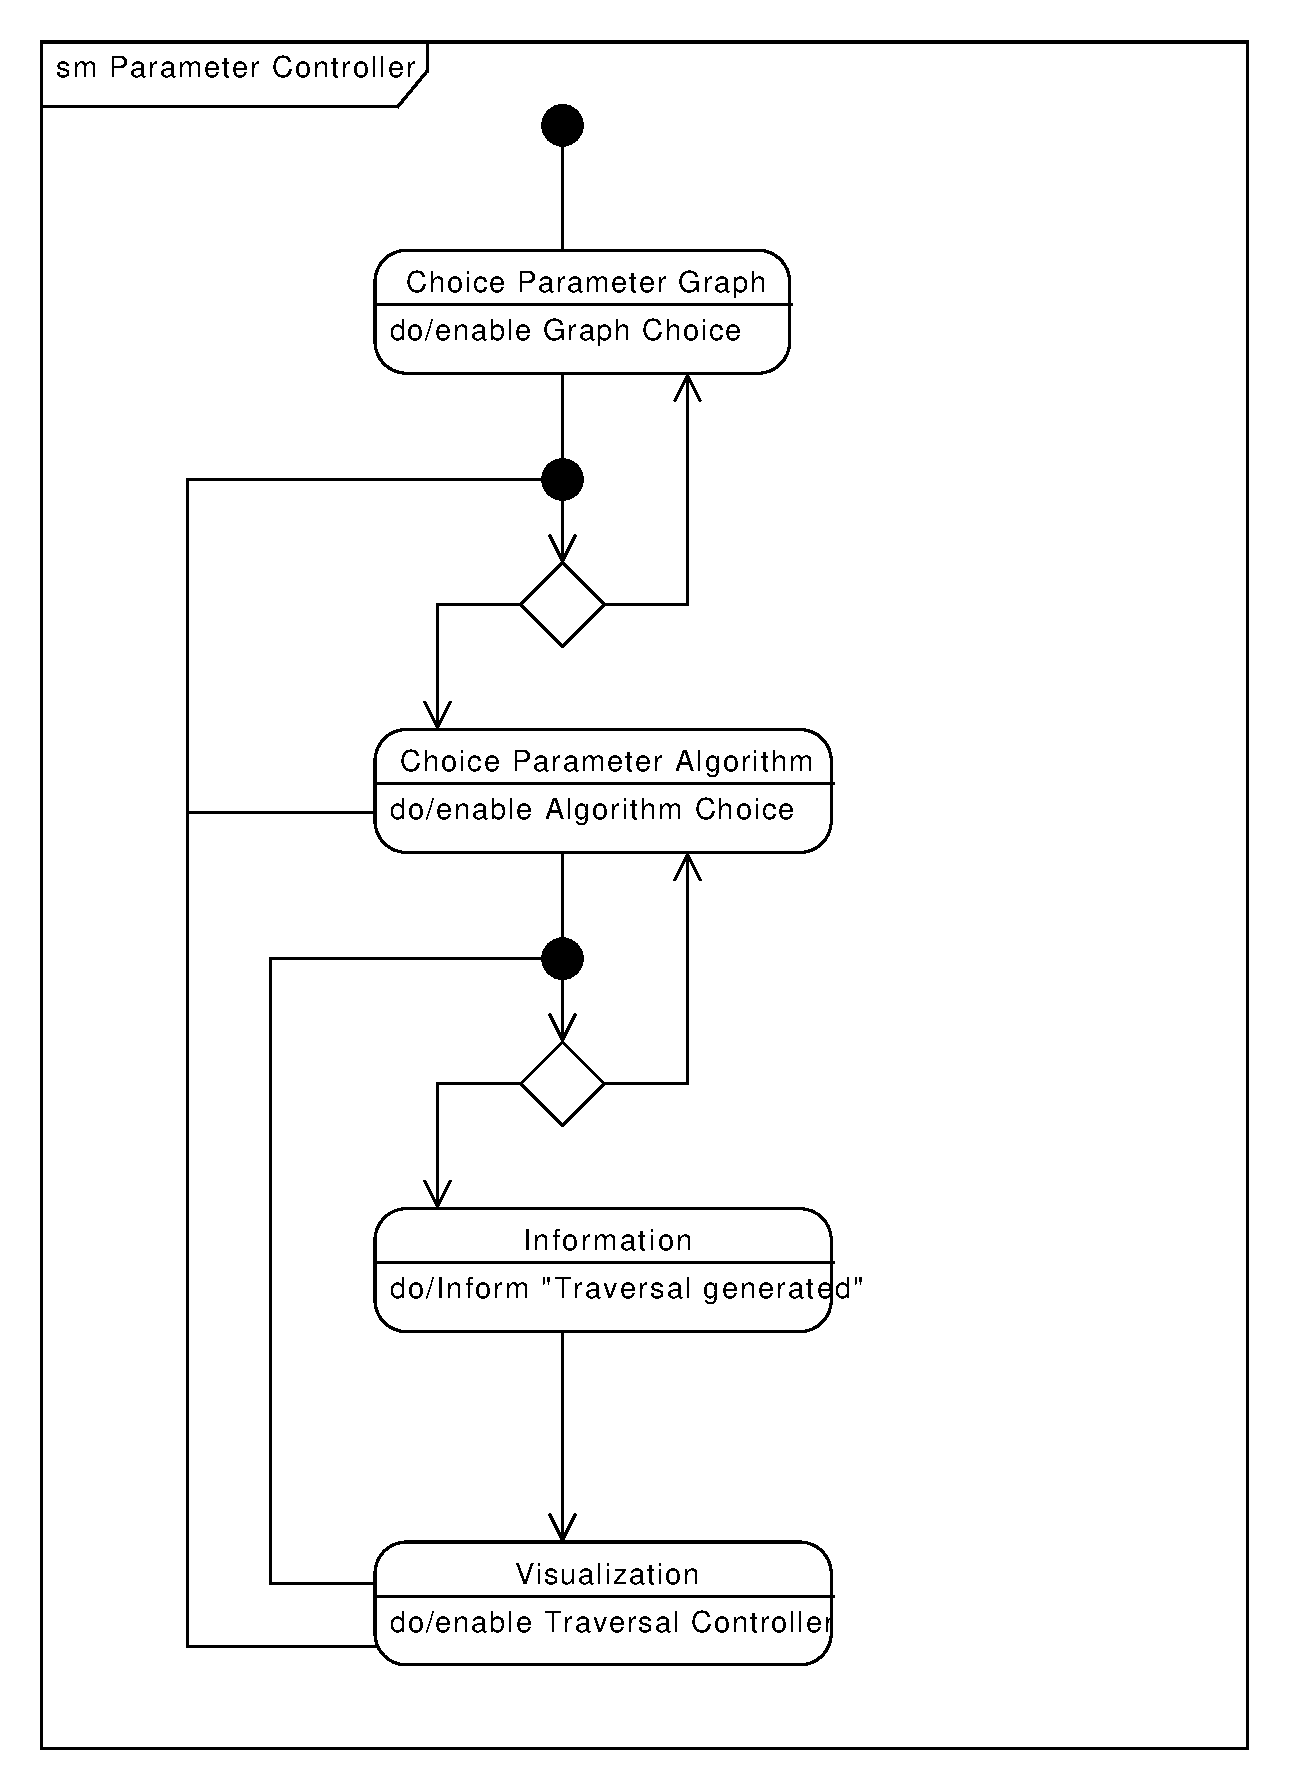
\includegraphics[
% 		    width=\textwidth,
% 		    height=\textheight,
% 		    angle=90,
		    scale=0.6,
		    keepaspectratio=true
    ]{diagrams/designmodel/sm-parameter-controller.pdf}
    \caption{Parameter Controller, State Diagram}
    \label{fig:parameter-controller-sm}
\end{figure}
% ----------------------------------------------------------------------------
% \newpage
% 
\subsection{Traversal Controller}
\begin{figure}[H]
    \centering
    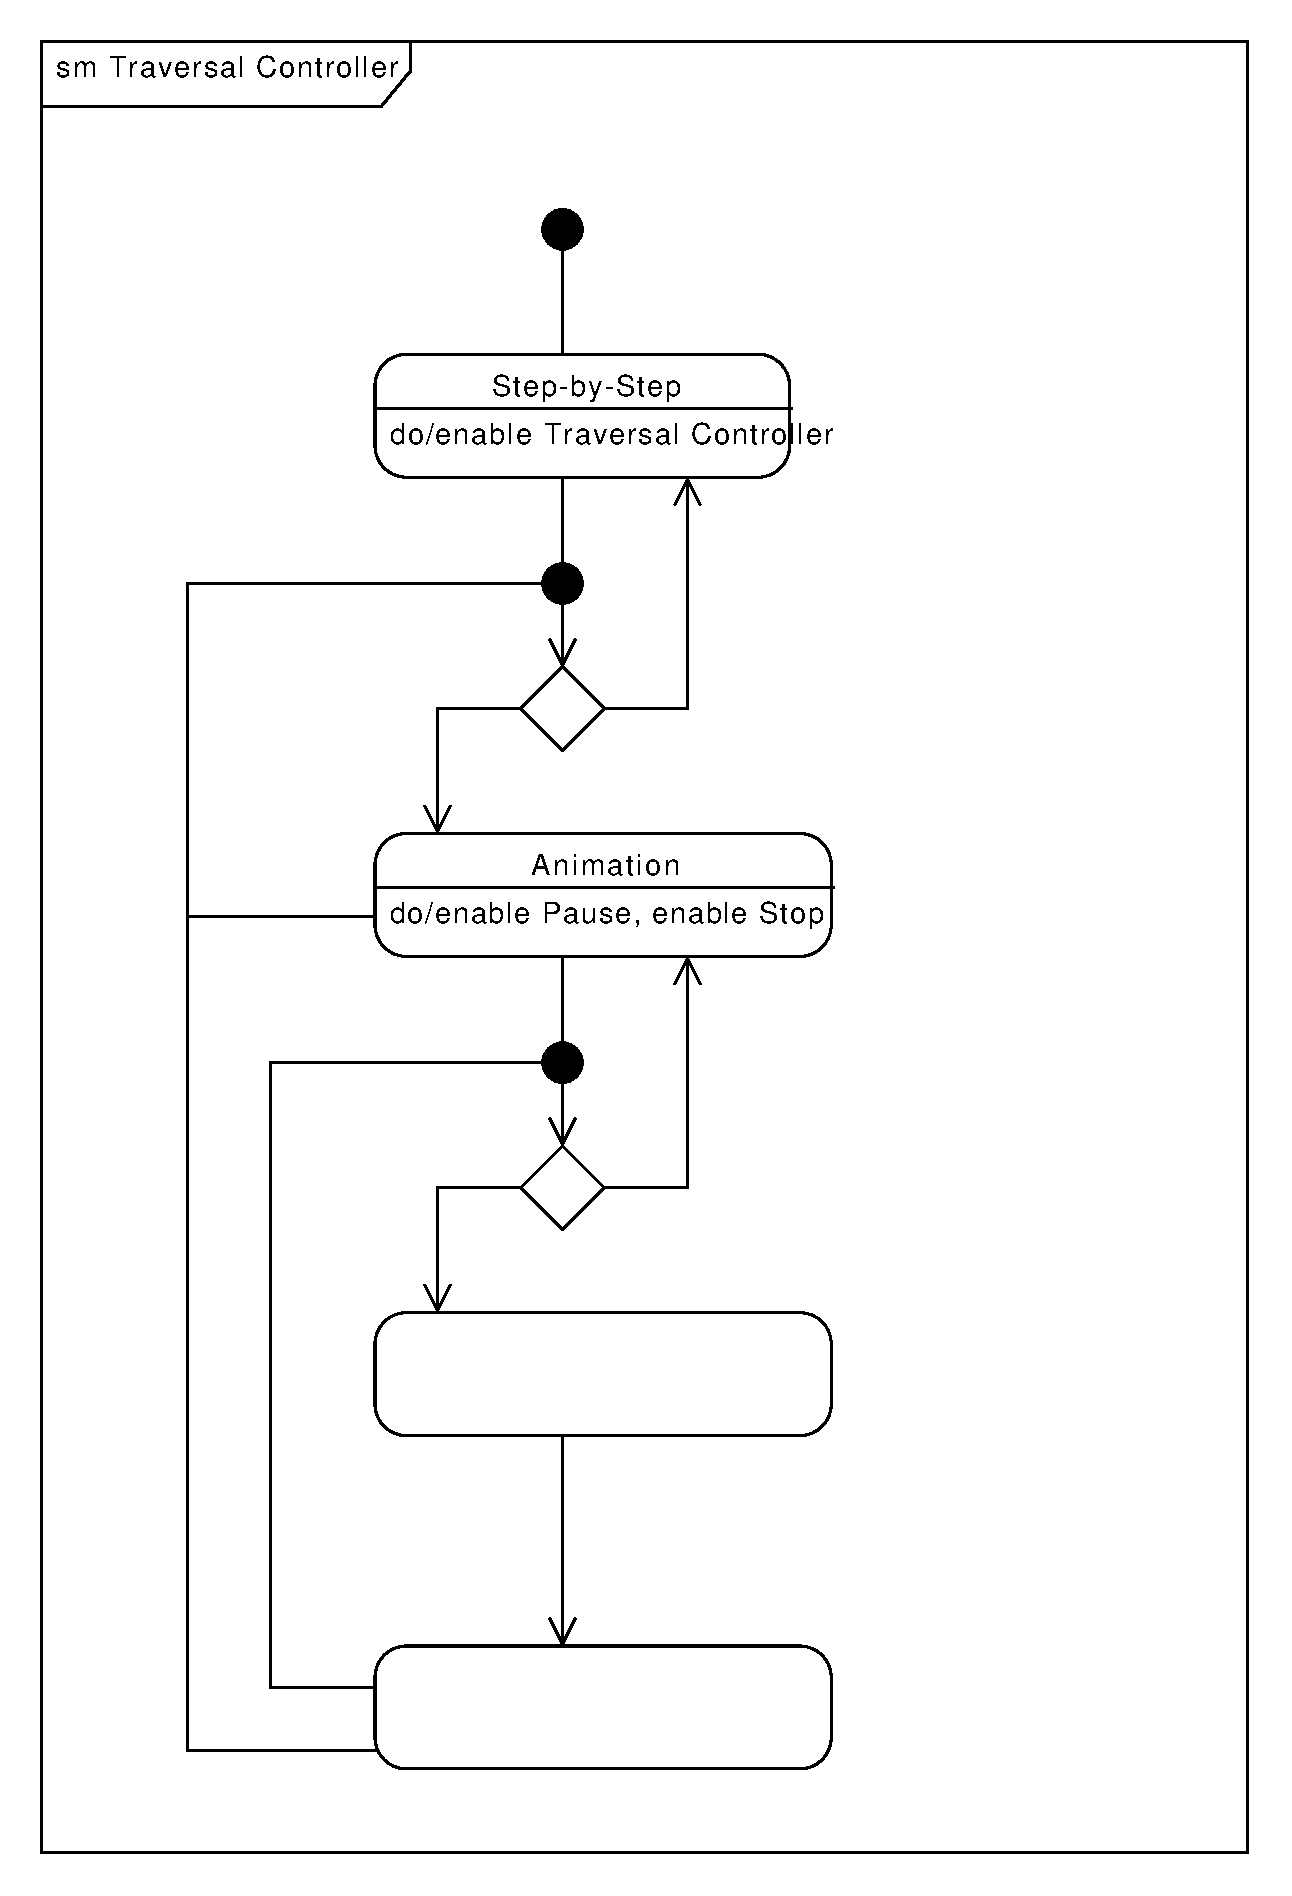
\includegraphics[
		    width=\textwidth,
% 		    height=\textheight,
% 		    angle=90,
		    scale=0.5,
		    keepaspectratio=true
%     ]{diagrams/designmodel/sm-traversal-controller.pdf}
    ]{diagrams/designmodel/sm-traversal-controller_draft_v2.jpeg}
    \caption{Traversal Controller, State Diagram}
    \label{fig:traversal-controller-sm}
\end{figure}
% ----------------------------------------------------------------------------
% \newpage
% 
\subsection{UC1 Import Graph}
\begin{figure}[H]
    \centering
    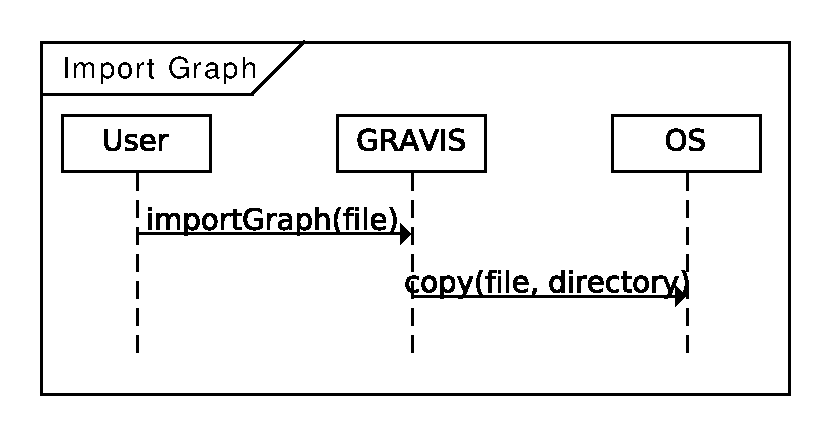
\includegraphics[
% 		    width=\textwidth,
% 		    height=\textheight,
% 		    angle=90,
		    scale=0.5,
		    keepaspectratio=true
	]{diagrams/designmodel/ssd-import-graph.pdf}
    \caption{UC1 Import Graph, System Sequence Diagram}
    \label{fig:import-graph-ssd}
\end{figure}
% \newpage
\begin{figure}[p]% will be the left-side figure
  \begin{leftfullpage}
    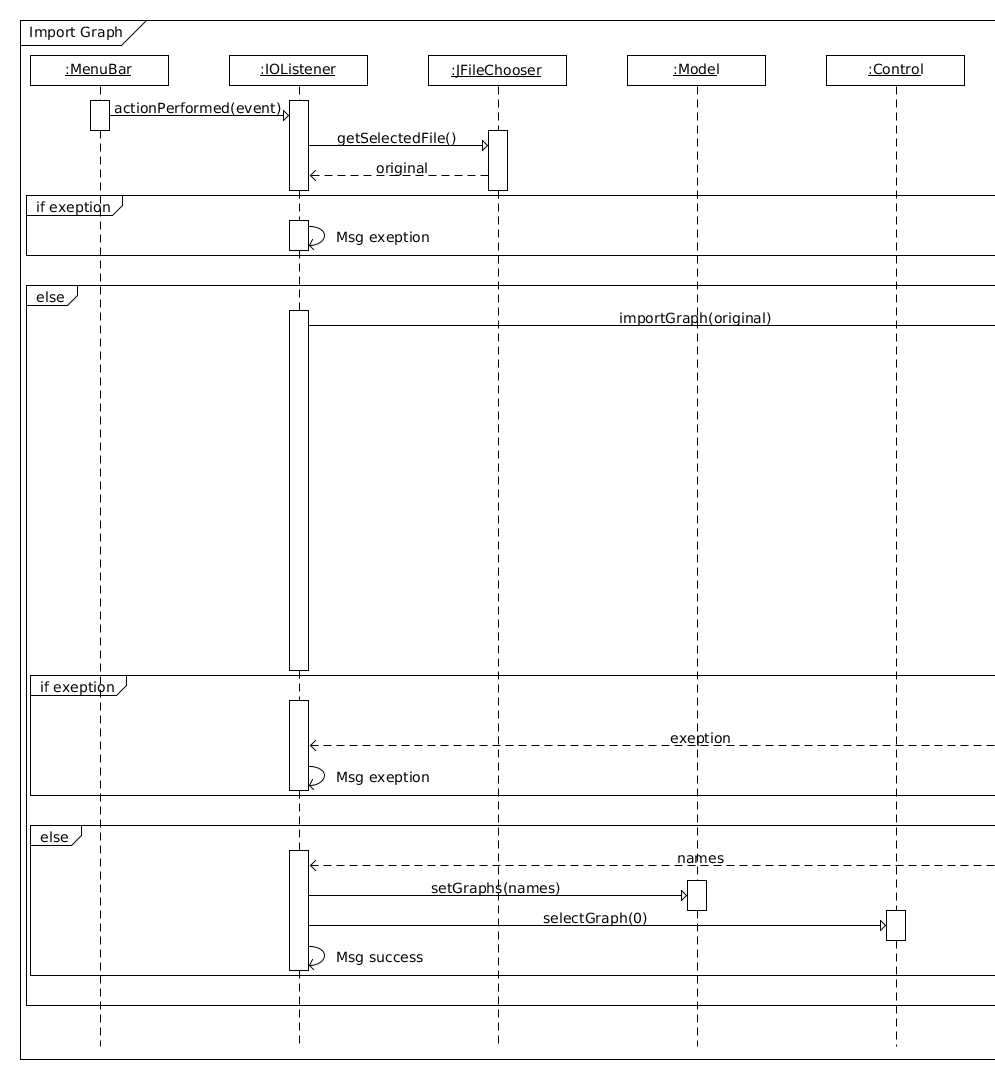
\includegraphics[
% 		    width=\textwidth,
% 		    height=\textheight,
% 		    angle=90,
		    scale=0.42,
% 		    keepaspectratio=true
	]{diagrams/designmodel/sd-import-graph-1-2.png}
    \caption{UC1 Import Graph, Sequence Diagram 1/2}
    \label{fig:import-graph-sd-1}
  \end{leftfullpage}
\end{figure}
\begin{figure}[p]% will be the right-side figure
  \begin{fullpage}
    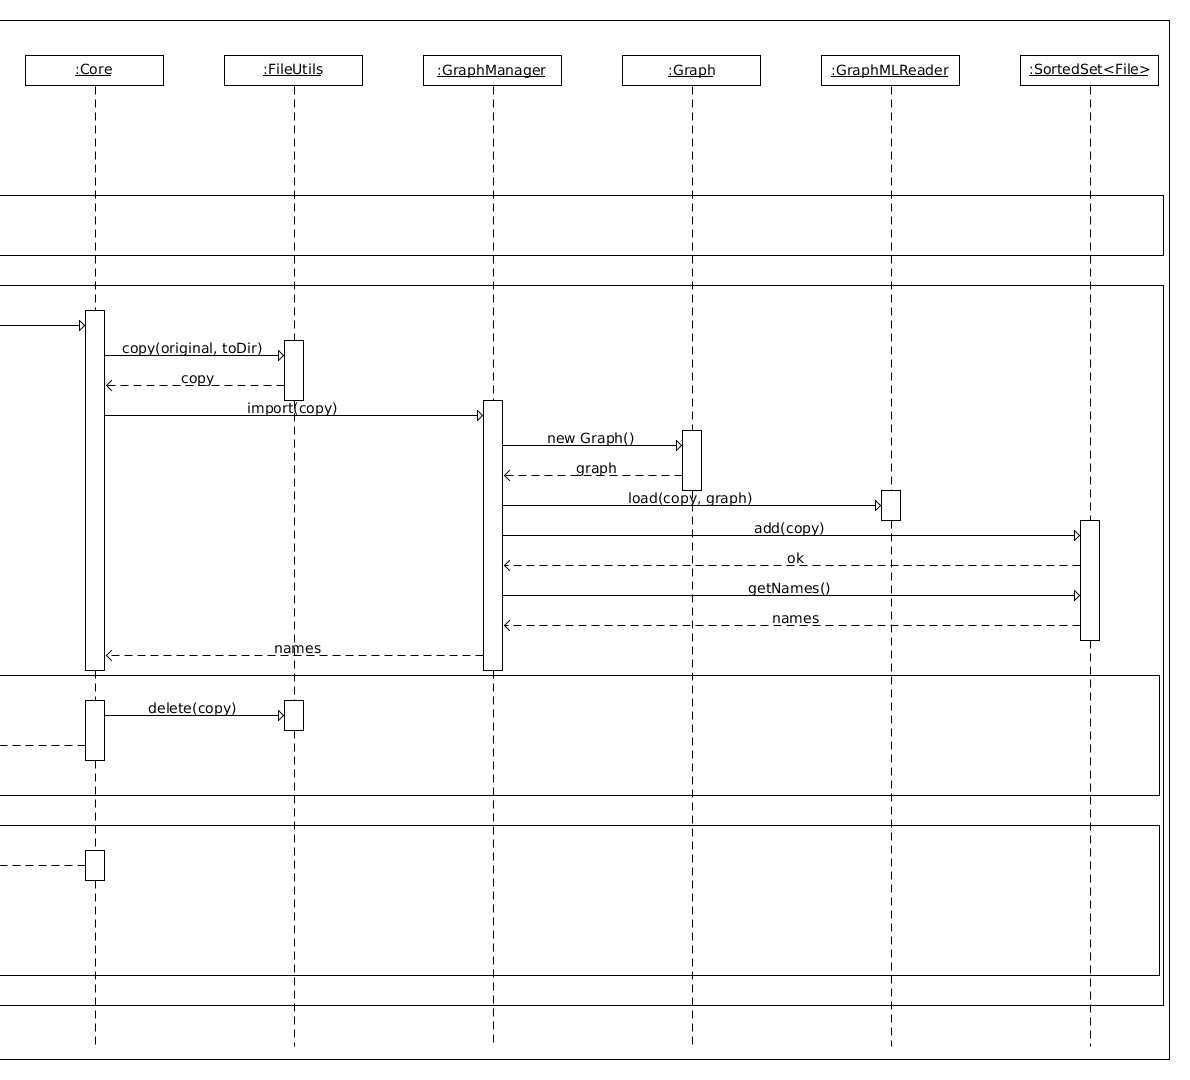
\includegraphics[
% 		    width=\textwidth,
% 		    height=\textheight,
% 		    angle=90,
		    scale=0.42,
% 		    keepaspectratio=true
	]{diagrams/designmodel/sd-import-graph-2-2.png}
    \caption{UC1 Import Graph, Sequence Diagram 2/2}
    \label{fig:import-graph-sd-2}
  \end{fullpage}
\end{figure}
% \newpage
\begin{figure}[H]
    \centering
    \includegraphics[width=\textwidth]{diagrams/designmodel/dcd-import-graph.pdf}
    \caption{UC1 Import Graph, Design Class Diagram}
    \label{fig:import-graph-dcd}
\end{figure}
% ----------------------------------------------------------------------------
% \newpage
% 
\subsection{UC2 Import Algorithm}
\begin{figure}[H]
    \centering
    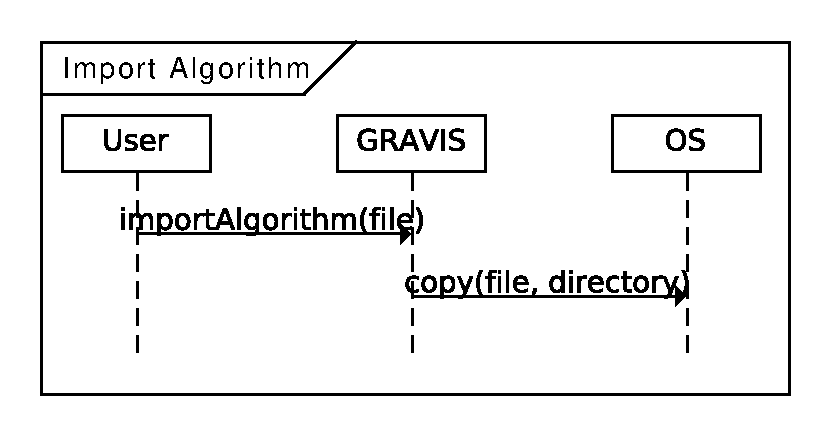
\includegraphics[
% 		    width=\textwidth,
% 		    height=\textheight,
% 		    angle=90,
		    scale=0.5,
		    keepaspectratio=true
      ]{diagrams/designmodel/ssd-import-algorithm.pdf}
    \caption{UC2 Import Algorithm, System Sequence Diagram}
    \label{fig:import-algorithm-ssd}
\end{figure}
% \newpage
\begin{figure}[p]% will be the left-side figure
  \begin{leftfullpage}
    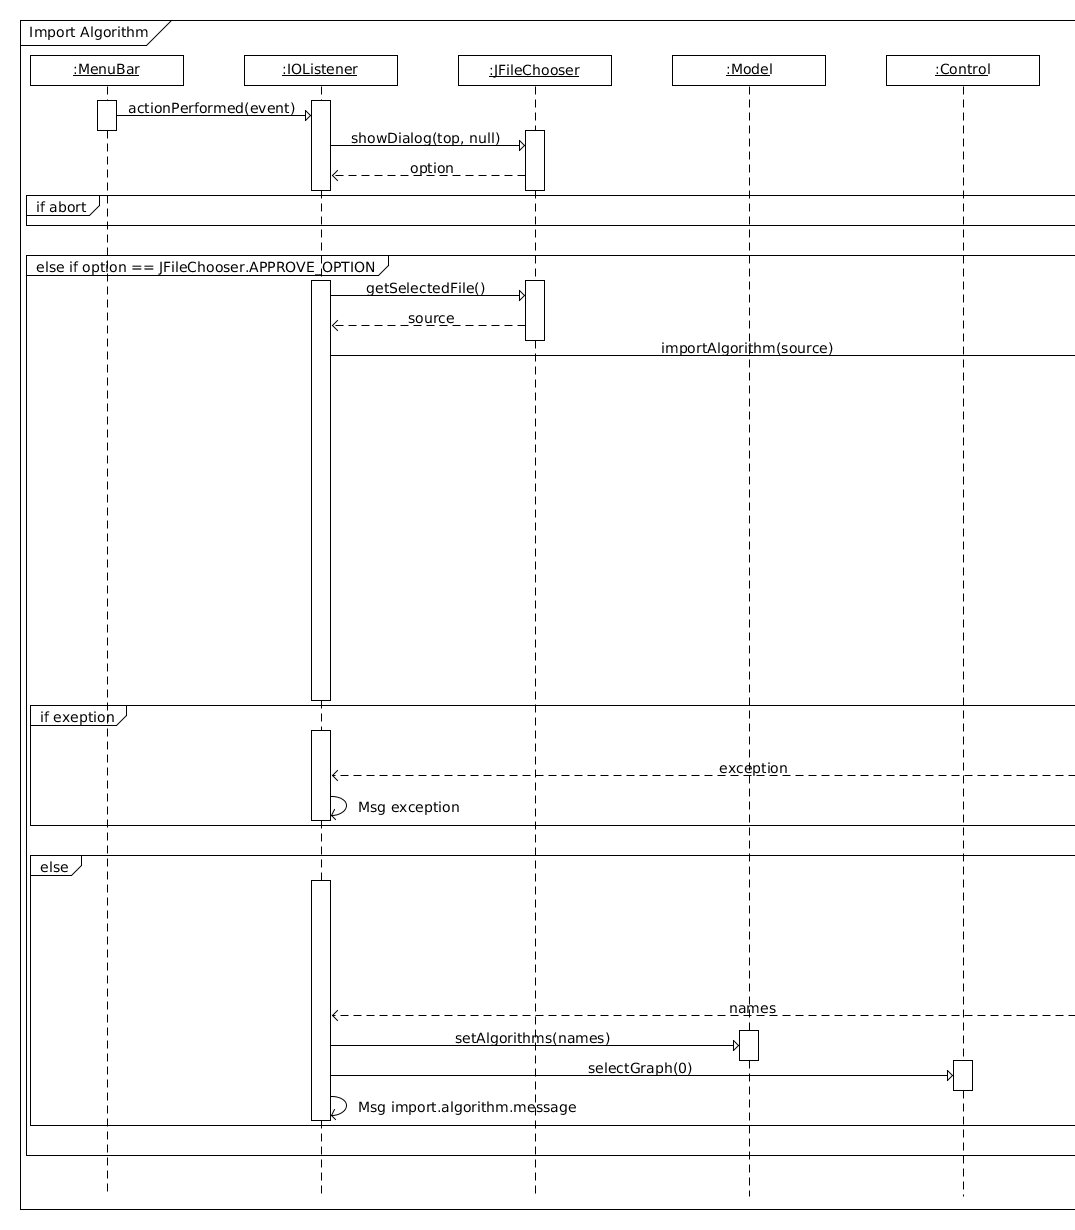
\includegraphics[
% 		    width=\textwidth,
% 		    height=\textheight,
% 		    angle=90,
		    scale=0.42,
% 		    keepaspectratio=true
	]{diagrams/designmodel/sd-import-algorithm-1-2.png}
    \caption{UC2 Import Algorithm, Sequence Diagram 1/2}
    \label{fig:import-algorithm-sd-1}
  \end{leftfullpage}
\end{figure}
\begin{figure}[p]% will be the right-side figure
  \begin{fullpage}
    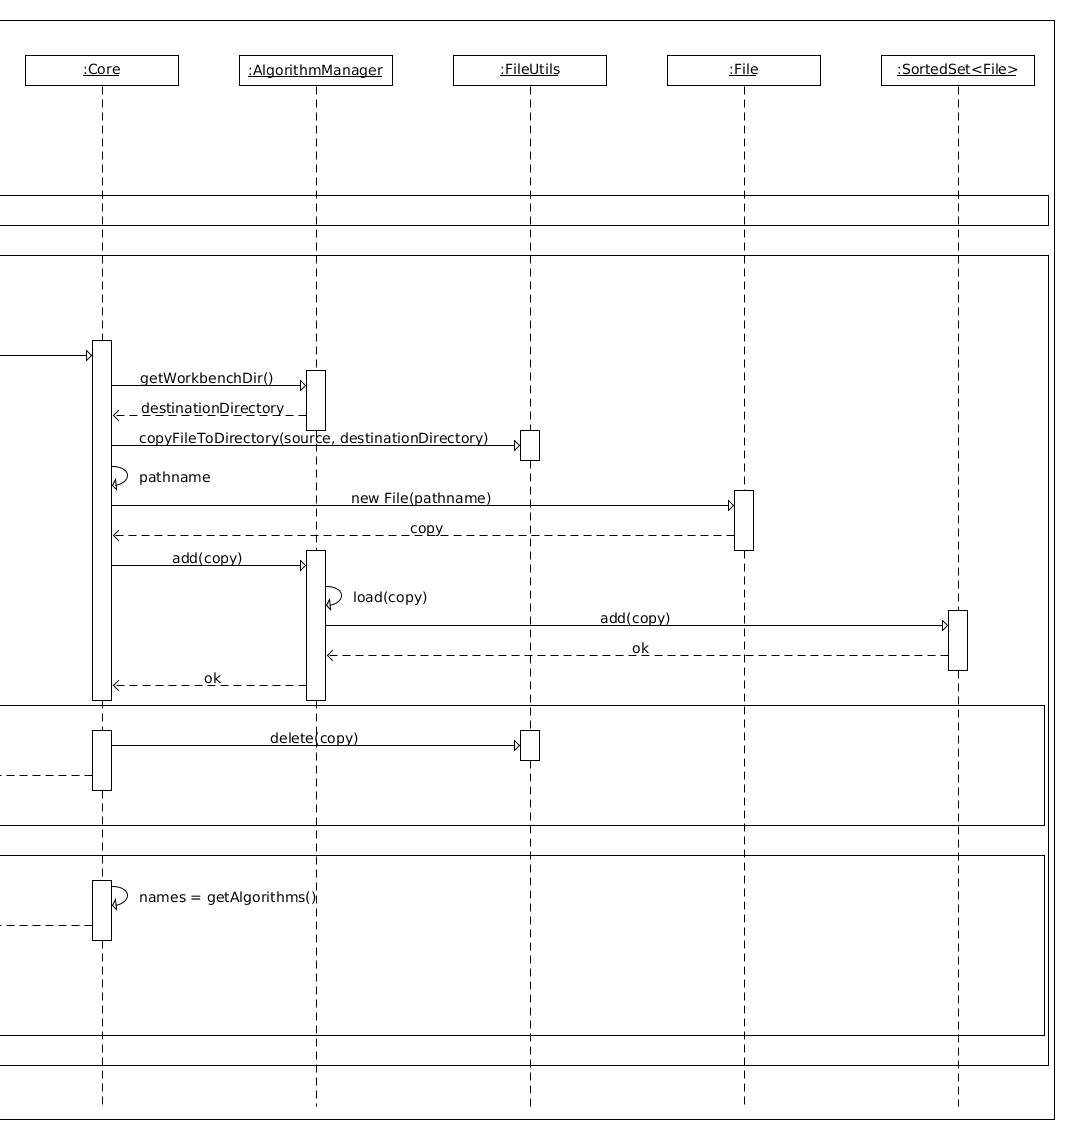
\includegraphics[
% 		    width=\textwidth,
% 		    height=\textheight,
% 		    angle=90,
		    scale=0.42,
% 		    keepaspectratio=true
	]{diagrams/designmodel/sd-import-algorithm-2-2.png}
    \caption{UC2 Import Algorithm, Sequence Diagram 2/2}
    \label{fig:import-algorithm-sd-2}
  \end{fullpage}
\end{figure}
% \newpage
\begin{figure}[H]
    \centering
    \includegraphics[width=\textwidth]{diagrams/designmodel/dcd-import-algorithm.pdf}
    \caption{UC2 Import Algorithm, Design Class Diagram}
    \label{fig:import-algorithm-dcd}
\end{figure}
% ----------------------------------------------------------------------------
% \newpage
% 
\subsection{UC3 Delete Graph}
\begin{figure}[H]
    \centering
    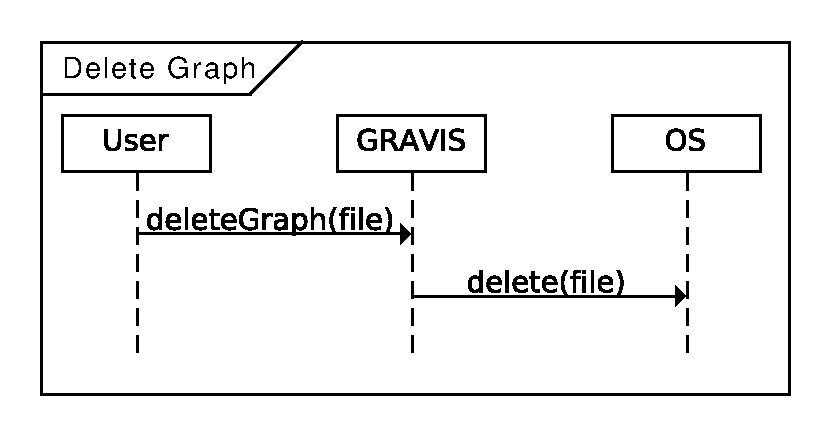
\includegraphics[
% 		    width=\textwidth,
% 		    height=\textheight,
% 		    angle=90,
		    scale=0.5,
		    keepaspectratio=true
      ]{diagrams/designmodel/ssd-delete-graph.pdf}
    \caption{UC3 Delete Graph, System Sequence Diagram}
    \label{fig:delete-graph-ssd}
\end{figure}
% \newpage
\begin{figure}[p]% will be the left-side figure
  \begin{leftfullpage}
    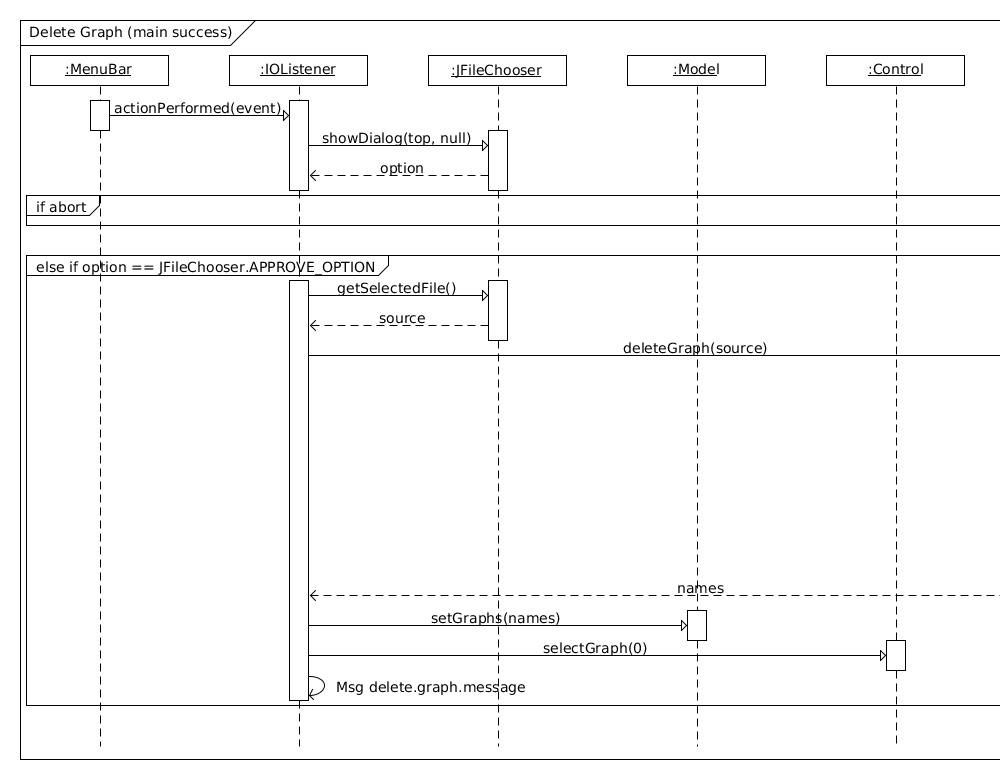
\includegraphics[
% 		    width=\textwidth,
% 		    height=\textheight,
% 		    angle=90,
		    scale=0.42,
% 		    keepaspectratio=true
	]{diagrams/designmodel/sd-delete-graph-1-2.png}
    \caption{UC3 Delete Graph, Sequence Diagram 1/2}
    \label{fig:delete-graph-sd-1}
  \end{leftfullpage}
\end{figure}
\begin{figure}[p]% will be the right-side figure
  \begin{fullpage}
    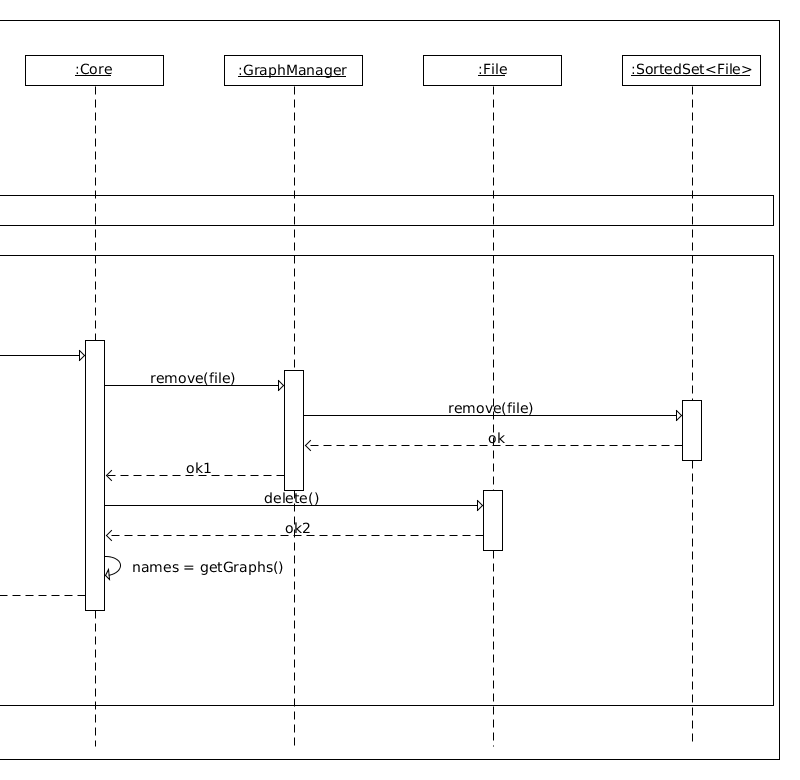
\includegraphics[
% 		    width=\textwidth,
% 		    height=\textheight,
% 		    angle=90,
		    scale=0.42,
% 		    keepaspectratio=true
	]{diagrams/designmodel/sd-delete-graph-2-2.png}
    \caption{UC3 Delete Graph, Sequence Diagram 2/2}
    \label{fig:delete-graph-sd-2}
  \end{fullpage}
\end{figure}
% \newpage
\begin{figure}[H]
    \centering
    \includegraphics[width=\textwidth]{diagrams/designmodel/dcd-delete-graph.pdf}
    \caption{UC3 Delete Graph, Design Class Diagram}
    \label{fig:delete-graph-dcd}
\end{figure}
% ----------------------------------------------------------------------------
% \newpage
% 
\subsection{UC4 Delete Algorithm}
\begin{figure}[H]
    \centering
    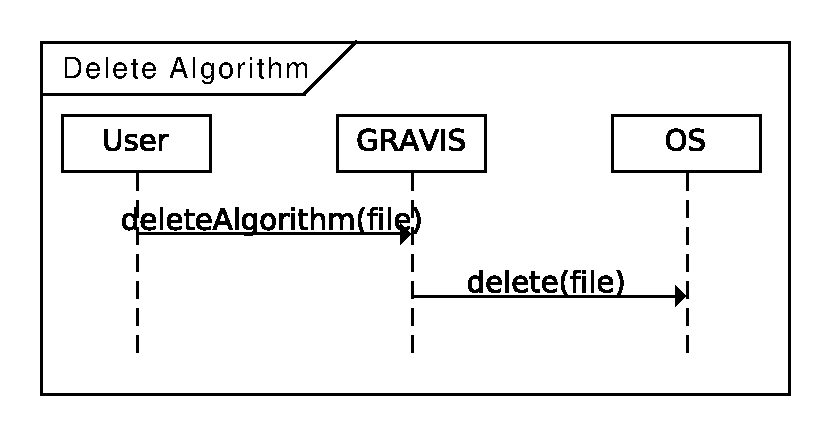
\includegraphics[
% 		    width=\textwidth,
% 		    height=\textheight,
% 		    angle=90,
		    scale=0.5,
		    keepaspectratio=true
      ]{diagrams/designmodel/ssd-delete-algorithm.pdf}
    \caption{UC4 Delete Algorithm, System Sequence Diagram}
    \label{fig:delete-algorithm-ssd}
\end{figure}
% \newpage
\begin{figure}[p]% will be the left-side figure
  \begin{leftfullpage}
    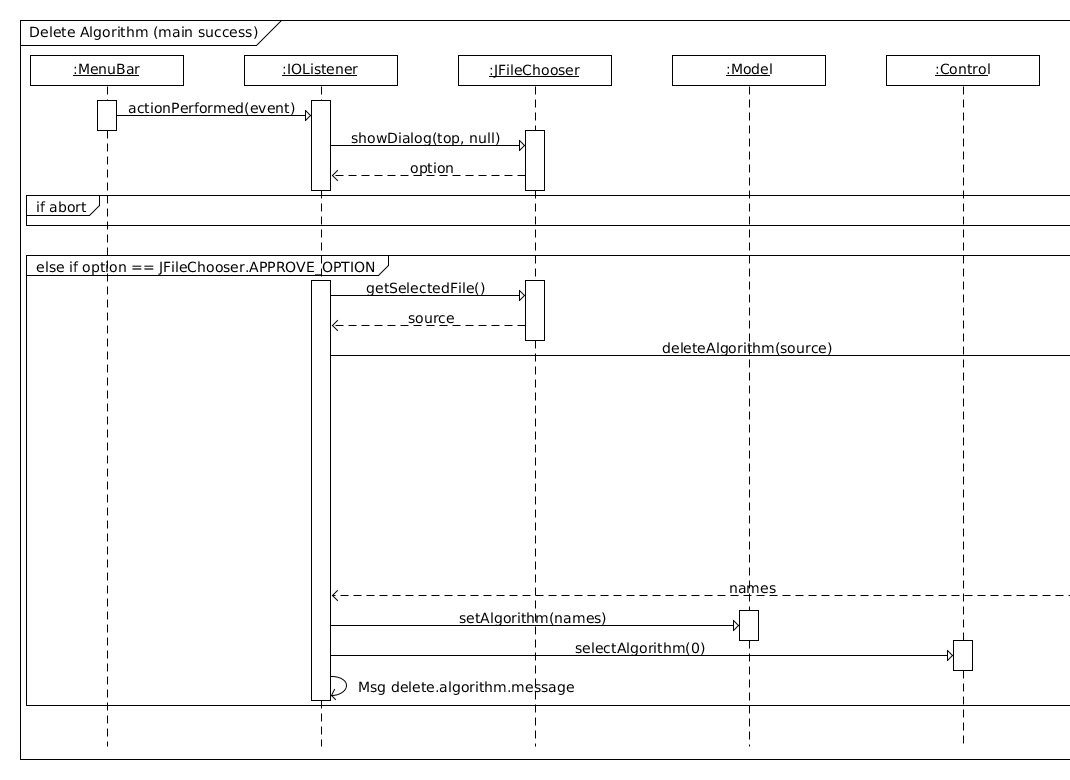
\includegraphics[
% 		    width=\textwidth,
% 		    height=\textheight,
% 		    angle=90,
		    scale=0.42,
% 		    keepaspectratio=true
	]{diagrams/designmodel/sd-delete-algorithm-1-2.png}
    \caption{UC4 Delete Algorithm, Sequence Diagram 1/2}
    \label{fig:delete-algorithm-sd-1}
  \end{leftfullpage}
\end{figure}
\begin{figure}[p]% will be the right-side figure
  \begin{fullpage}
    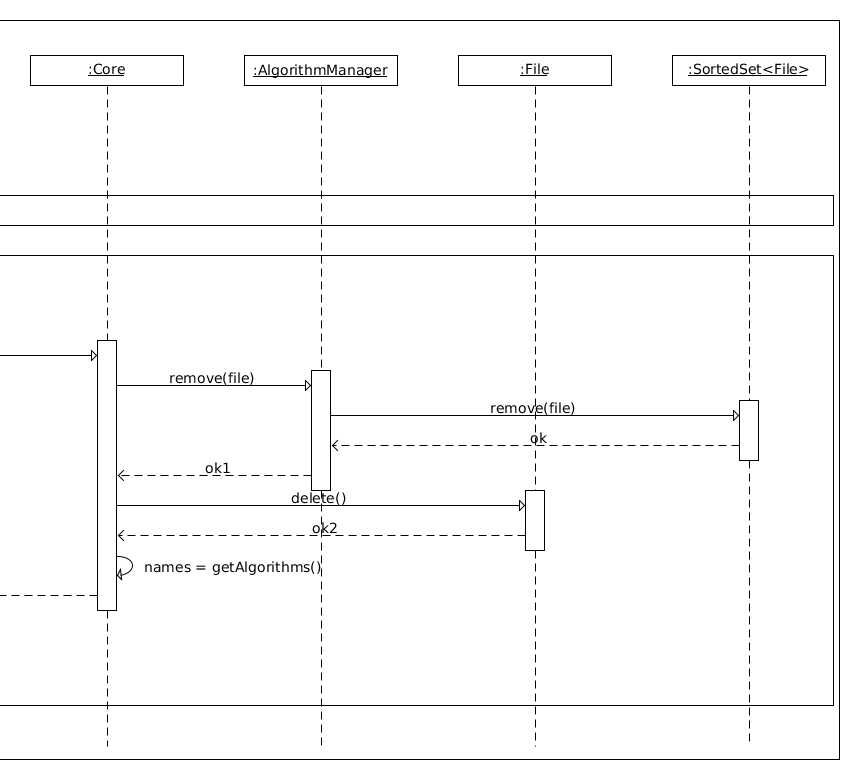
\includegraphics[
% 		    width=\textwidth,
% 		    height=\textheight,
% 		    angle=90,
		    scale=0.42,
% 		    keepaspectratio=true
	]{diagrams/designmodel/sd-delete-algorithm-2-2.png}
    \caption{UC4 Delete Algorithm, Sequence Diagram 2/2}
    \label{fig:delete-algorithm-sd-2}
  \end{fullpage}
\end{figure}
% \newpage
\begin{figure}[H]
    \centering
    \includegraphics[width=\textwidth]{diagrams/designmodel/dcd-delete-algorithm.pdf}
    \caption{UC4 Delete Algorithm, Design Class Diagram}
    \label{fig:delete-algorithm-dcd}
\end{figure}
% ----------------------------------------------------------------------------
% \newpage
% 
\subsection{UC5 Select Graph}
\begin{figure}[H]
    \centering
    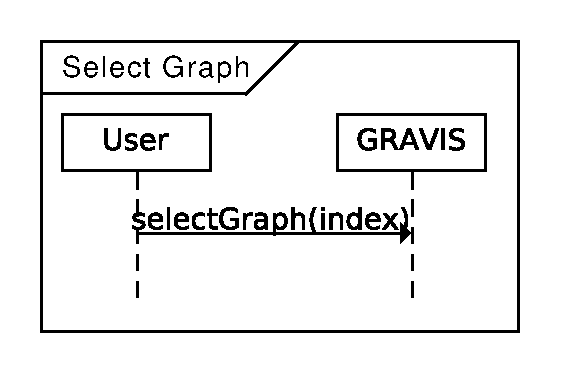
\includegraphics[
% 		    width=\textwidth,
% 		    height=\textheight,
% 		    angle=90,
		    scale=0.5,
		    keepaspectratio=true
      ]{diagrams/designmodel/ssd-select-graph.pdf}
    \caption{UC5 Select Graph, System Sequence Diagram}
    \label{fig:select-graph-ssd}
\end{figure}
% \newpage
\begin{figure}[p]% will be the left-side figure
  \begin{leftfullpage}
    \includegraphics[
% 		    width=\textwidth,
% 		    height=\textheight,
% 		    angle=90,
		    scale=0.42,
% 		    keepaspectratio=true
	]{diagrams/designmodel/sd-select-graph-1-2.png}
    \caption{UC5 Select Graph, Sequence Diagram 1/2}
    \label{fig:select-graph-sd-1}
  \end{leftfullpage}
\end{figure}
\begin{figure}[p]% will be the right-side figure
  \begin{fullpage}
    \includegraphics[
% 		    width=\textwidth,
% 		    height=\textheight,
% 		    angle=90,
		    scale=0.42,
% 		    keepaspectratio=true
	]{diagrams/designmodel/sd-select-graph-2-2.png}
    \caption{UC5 Select Graph, Sequence Diagram 2/2}
    \label{fig:select-graph-sd-2}
  \end{fullpage}
\end{figure}
% \newpage
\begin{figure}[H]
    \centering
    \includegraphics[width=\textwidth]{diagrams/designmodel/dcd-select-graph.pdf}
    \caption{UC5 Select Graph, Design Class Diagram}
    \label{fig:select-graph-dcd}
\end{figure}
% ----------------------------------------------------------------------------
% \newpage
% 
\subsection{UC6 Select Algorithm}
\begin{figure}[H]
    \centering
    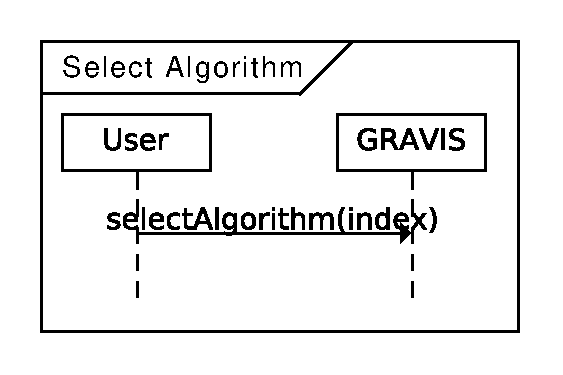
\includegraphics[
% 		    width=\textwidth,
% 		    height=\textheight,
% 		    angle=90,
		    scale=0.5,
		    keepaspectratio=true
      ]{diagrams/designmodel/ssd-select-algorithm.pdf}
    \caption{UC6 Select Algorithm, System Sequence Diagram}
    \label{fig:select-algorithm-ssd}
\end{figure}
% \newpage
\begin{figure}[p]% will be the left-side figure
  \begin{leftfullpage}
    \includegraphics[
% 		    width=\textwidth,
% 		    height=\textheight,
% 		    angle=90,
		    scale=0.42,
% 		    keepaspectratio=true
	]{diagrams/designmodel/sd-select-algorithm-1-2.png}
    \caption{UC6 Select Algorithm, Sequence Diagram 1/2}
    \label{fig:select-algorithm-sd-1}
  \end{leftfullpage}
\end{figure}
\begin{figure}[p]% will be the right-side figure
  \begin{fullpage}
    \includegraphics[
% 		    width=\textwidth,
% 		    height=\textheight,
% 		    angle=90,
		    scale=0.42,
% 		    keepaspectratio=true
	]{diagrams/designmodel/sd-select-algorithm-2-2.png}
    \caption{UC6 Select Algorithm, Sequence Diagram 2/2}
    \label{fig:select-algorithm-sd-2}
  \end{fullpage}
\end{figure}
% \newpage
\begin{figure}[H]
    \centering
    \includegraphics[width=\textwidth]{diagrams/designmodel/dcd-select-algorithm.pdf}
    \caption{UC6 Select Algorithm, Design Class Diagram}
    \label{fig:select-algorithm-dcd}
\end{figure}